\section*{Übung 8}
\subsection*{Aufgabe 1}
\subsubsection*{Lösungsidee}
Es sollen beliebig große ganze Zahlen addiert und multipliziert werden. Dazu wird eine Liste verwendet in der Nodes sind, die einen Integer mit maximal drei Stellen beinhalten. Diese Integer der Nodes zusammen gezählt ergeben die Zahl, wobei die erste Node die untersten drei Stellen der Zahl und die letzte Node die größten drei Stellen der Zahl beinhaltet. Für das Addieren und multiplizieren werden eigene Funktionen erstellt denen BigInPtr übergeben werden. Damit auch negative Zahlen addiert werden können, wird eine Funktion  HigherBigInt verwendet die zurückgibt welche Zahl größer ist bzw. ob beide gleich sind. Je nachdem was dies Funktion zurückliefert wird unterschiedlich gerechnet. Für das allgemeine Addieren werden die Integer der Nodes zusammen gezählt und mit einem overflow Integer zusammengezählt. Ist diese Summe größer als 999 muss bei der nächsten Node + 1 dazu gezählt werden, daher wird overflow auf 1 gesetzt. Bei negativen Zahlen wird überprüft ob die Summe unter 0 ist. Falls dies der Fall ist wird overflow auf -1 gesetzt und bei der nächsten Node subtrahiert.
\newline

\lstinputlisting[language=Pascal] {../BigInts.pas}
\begin{figure}[H]
	\centering
	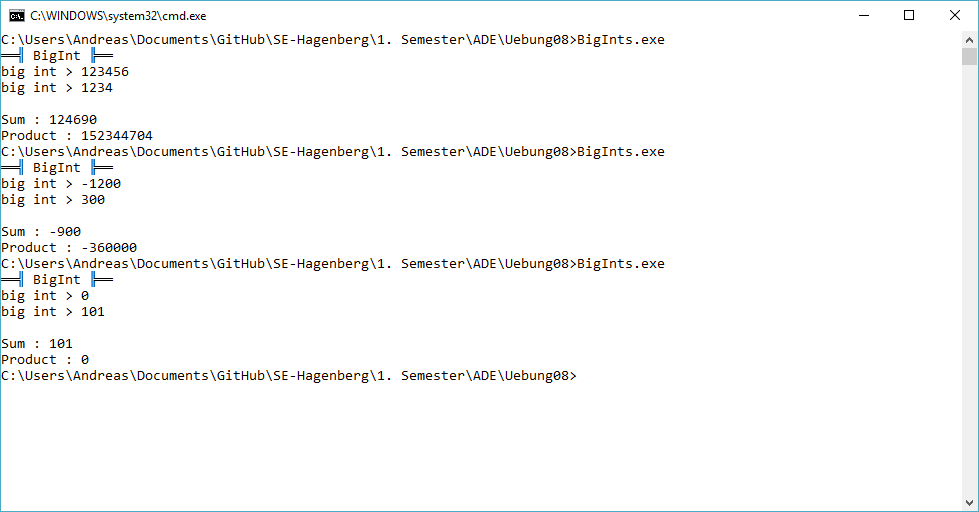
\includegraphics[scale=0.65]{./pictures/BigInts.png}
	\caption{Testfälle BigInts}
	\label{fig: BigInts}
\end{figure}

\section*{Testfälle}
Die Testfälle zeigen die Addition / Multiplikation mit positiven und negativen Zahlen. Das Addieren funktioniert solange genug Speicher für die Liste vorhanden ist. Beim Multiplizieren wird ein Laufzeitfehler verursacht wenn der Maximale Wertebereich von Int64 unter/überschritten wird. Alternativ kann hier mit einem String gearbeitet werden, jedoch ist dieser auch \grqq beschränkt\grqq{} auf 255 Zeichen,  \grqq unendlich lange\grqq{} Zahlen können damit aber nicht verwirklicht werden.
\newpage

\subsection*{Aufgabe 2}
\subsubsection*{Lösungsidee}
Bei dieser Aufgabe wird eine Wish List erstellt die Wünsche von einem Text Dokument einliest. Aufgrund dieser Liste wird eine Order Liste erstellt. In dieser sind alle Dinge die sich die Kinder wünschen Mengenmäßig enthalten. Danach wird eine Delivery Liste erstellt, in der alle Wünsche für das jeweilige Kind enthalten ist. Es werden für die Ausgabe, Node-erstellung und anfügen an eine Liste Funktionen bzw. Prozeduren erstellt.
\newline

\lstinputlisting[language=Pascal] {../WLA.pas}
\begin{figure}[H]
	\centering
	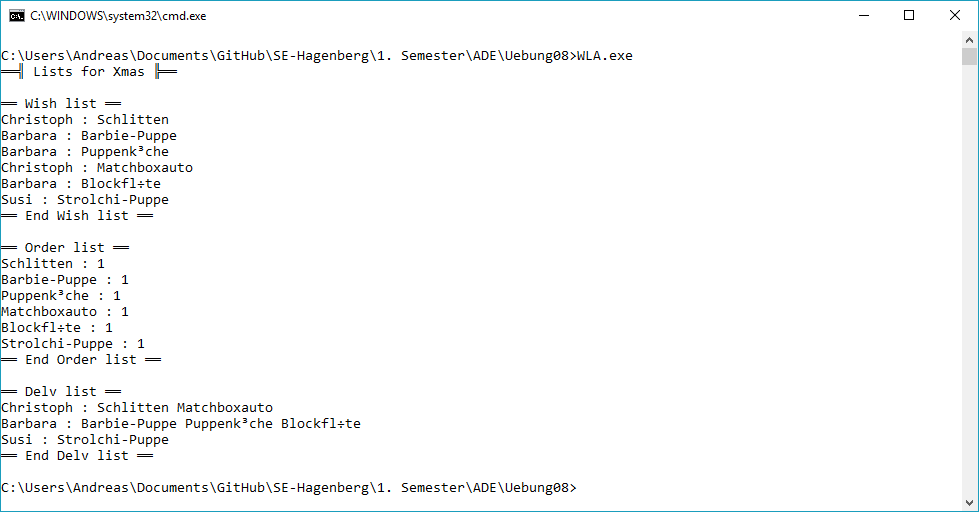
\includegraphics[scale=0.65]{./pictures/XMAS.png}
	\caption{Testfälle WLA}
	\label{fig: WLA}
\end{figure}

\section*{Testfall}
Hier wird gezeigt, dass die WishList die Wünsche der Kinder aus dem Textdokument enthält. Die OrderList wird aufgrund dieser Liste erzeugt. Die DeliveryList enthält Kinder mit ihren Wünschen basierend auf der WishList.
\newpage



